\graphicspath{{./Ch3-CNN/images/}}

\chapter{Optimizing the Performance of CNN Accelerators} \label{chap:CNN}
CNNs are the state of the art machine learning algorithms. CNNs can achieve human-like accuracy in computer vision-related tasks. In order to achieve high accuracy, modern CNNs use a deep hierarchy of layers and perform compute-intensive and memory-intensive operations. CNN accelerators use many processing elements to exploit parallelism to speed up the computations. However, limited off-chip memory bandwidth limits their performance. In addition, considerable data transfer volume from the off-chip memory also results in high energy consumption.

CNNs have a sequence of mainly three types of layers: convolution layer (CL), pooling layer, and fully connected layer (FCL). There are several CLs, and a pooling layer usually follows each CL. The last few layers of the CNNs are FCLs. VGG16 has thirteen CLs, and the last three layers are FC. Similarly, AlexNet has five CLs, followed by 3 FCLs. Pooling layer computations involve sliding a two-dimensional filter window over a single channel of \textit{ifm} and selecting one activation from the window using an operation like maximum or average. There are no parameters in pooling layers. The pooling layer helps reduce the activation sizes and, thus, the number of parameters in subsequent layers. CL and FC layers are compute-intensive, requiring millions of parameters. 

\figref{fig:CLOps} and~\figref{fig:FCLOps} illustrate the computations of a CL and an FCL, respectively. Each CL and FCL layer takes 3D input frames (\textit{ifm}) and applies filter weights (\textit{wts}) to compute output frames (\textit{ofm}). 3D $ifm$, $wts$ and $ofm$ are composed of $2D$ matrices stacked together in depth dimension. The number of 2D matrices is referred to as channels or depth of the data type. The number of channels ($N_i$) in each filter and $ifm$ are the same.

The convolution is performed by element-wise product between $K{\times}K$ filter elements with a 2D window of $ifm$ of size $K{\times}K$, for all the $N_i$ channels and then adding resulting $K{\times}K{\times}N_i$ elements to compute one element of the $ofm$ channel. Other elements of the $ofm$ channel are computed by sliding the 2D filter over the spatial dimension of the $ifm$ ($H_i{\times}W_i$). Filter slides by S elements from left to right and then top to bottom. $K$ and $S$ are referred to as the filter size and stride of the filter, respectively. We assumed square filters of dimension $K{\times}K$, $K$ is an odd integer, filter stride in horizontal and vertical directions are identical, and $S{\le}K$, which are typically the case. 

\begin{figure}[!htb]
	\centering
	\captionsetup{font=sf}	
	\subfloat[Convolution Layer]{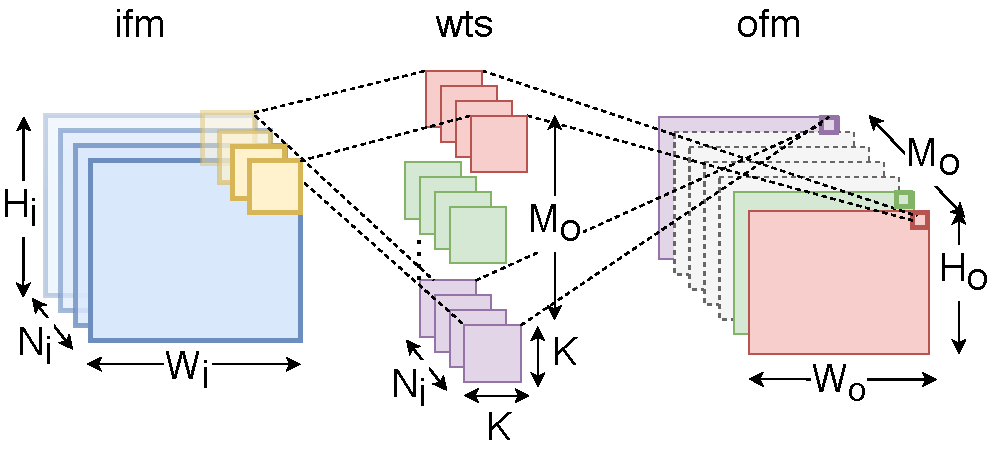
\includegraphics[width=0.49\textwidth]{CLOps.pdf}
		\label{fig:CLOps}}
	\hfil	
	\subfloat[Fully Connected Layer]{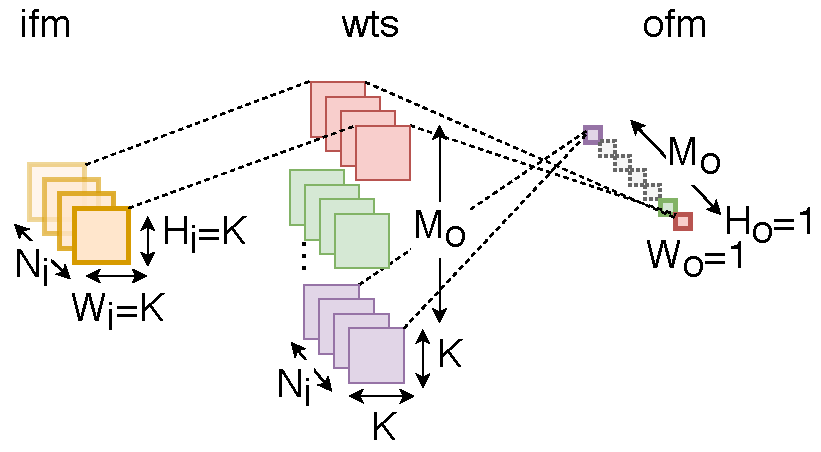
\includegraphics[width=0.42\textwidth]{FCLOps.pdf}
		\label{fig:FCLOps}}
	\hfil	
	\caption{Convolution and fully connected layers}
	\label{fig:CNNAcceleratorAndCLOps}
\end{figure}

$ofm$ dimensions of CL and FC layers can be computed using the $ifm$ dimensions, filter size ($K$), and stride ($S$). \figref{fig:CLInOutDimRel} illustrates the relation of ofm dimension with ifm and filter dimensions for stride $S{=}1$. The filter can be placed at $W_i{-}(K{-}1)$ horizontal locations and $H_i{-}(K{-}1)$ locations in the vertical dimensions of the $ifm$. If $S{=}1$, the $ofm$ spatial dimensions are $K{-}1$ elements less than the $ifm$ dimensions. Several CNN architectures add padding elements to the border of the $ifm$ spatial dimensions. If the padding on the left, right, top, and bottom are $P_l$, $P_r$, $P_t$, and $P_b$, respectively, the $ofm$ dimensions for $S{=}1$ can be computed as follows,
\begin{align}\label{eq:ifmOfmStrideOne}
	\begin{split}
W_o&=W_i+P_l+P_r-(K-1)\\
H_o&=H_i+P_t+P_b-(K-1)
\end{split}
\end{align}
\begin{figure}[!htb]
	\centering
	\captionsetup{font=sf}	
	{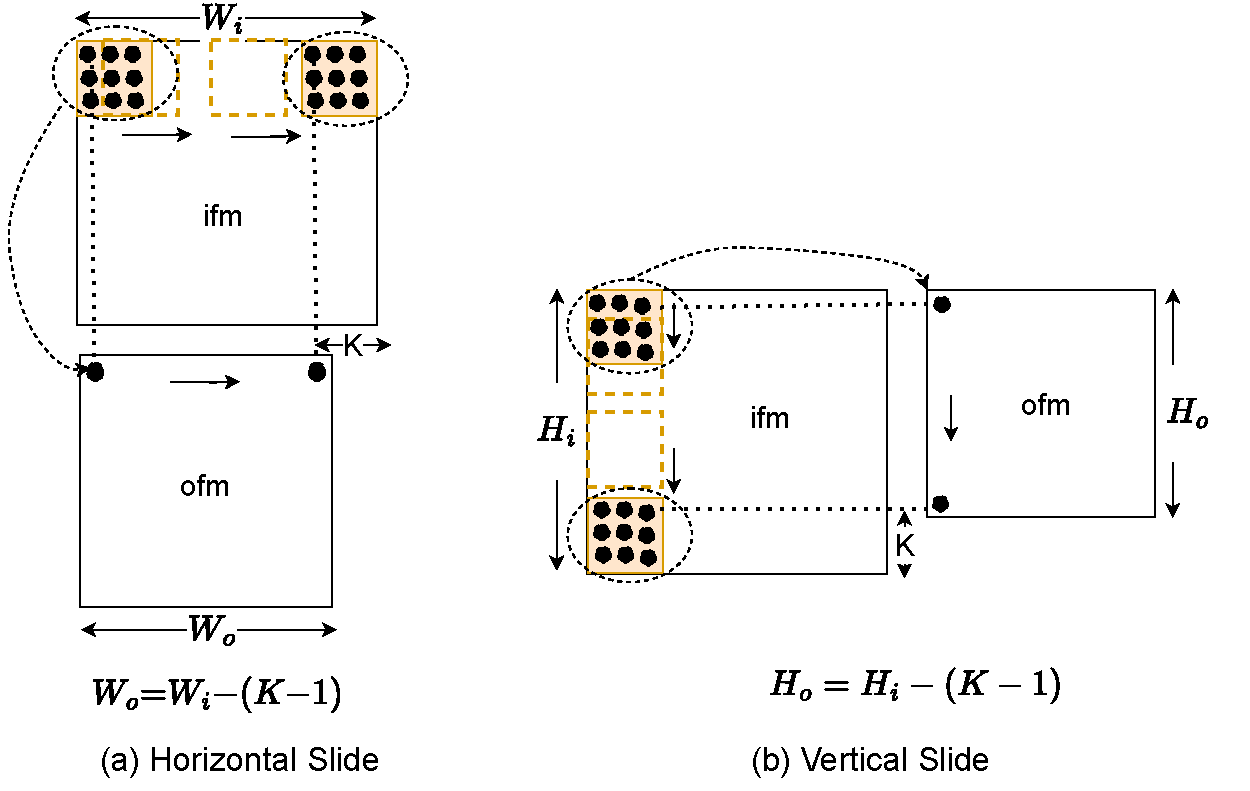
\includegraphics[width=0.8\textwidth]{convInAndOutDims.pdf}
		\label{fig:CLInOutRelHz}}
	\caption{Input and Output dimensions of CL layer for filter stride=1  }
	\label{fig:CLInOutDimRel}
\end{figure}
If the stride is not 1, the number of elements in the $ofm$ spatial dimensions reduces by a factor of $S$. If the filter stride is $S$, $ofm$ spatial dimensions can be expressed as follows, which is the generalization of the equation~\eqref{eq:ifmOfmStrideOne}
\begin{align}\label{eq:ifmOfmStrideS}
	\begin{split}
		W_o&=\ceil[\big]{\frac{W_i+P_l+P_r-(K-1)}{S}}\\
		H_o&=\ceil[\big]{\frac{H_i+P_t+P_b-(K-1)}{S}}
	\end{split}
\end{align}
If the padding at the top, bottom, left and right are the same as $P$, ~\eqref{eq:ifmOfmStrideS} can be simplified as follows,
\begin{align}\label{eq:ifmOfmStrideS_P}
	\begin{split}
		W_o&={\frac{W_i+2\cdot P-K}{S}}{+}1\\
		H_o&={\frac{H_i+2\cdot P-K}{S}{+}1}
	\end{split}
\end{align}

CNN accelerators have limited on-chip memory size. Layer activations and parameter sizes are too large to fit into the on-chip memory. CNN accelerators apply loop tiling to partition the layer data into small tiles that fit into on-chip memory. Loop tiling is a compiler  technique~\cite{aho2006compilers} that partitions the loop iteration space and large arrays into smaller tiles to increase the data locality and ensure data fits into smaller memories. \figref{fig:partitioningDataUsingTiling} shows a layer's data stored in off-chip memory and its tiles in the accelerator's on-chip buffer.
\begin{figure}[!htb]
	\centering
	\captionsetup{font=sf}	
	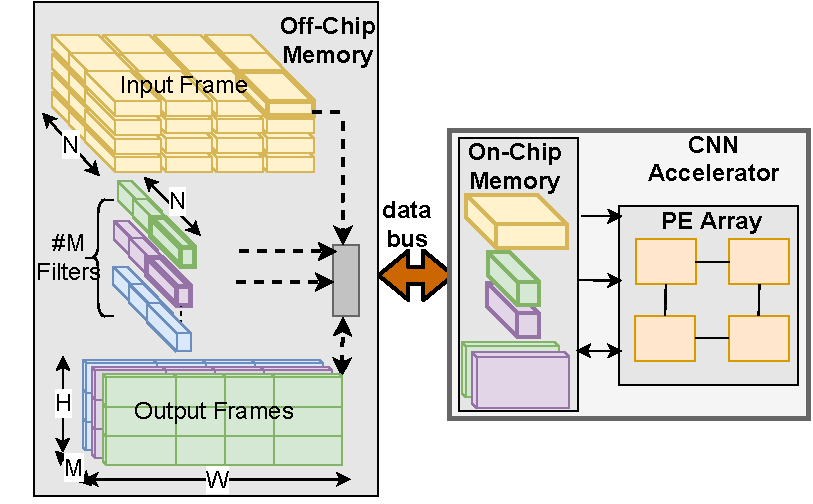
\includegraphics[width=0.5\textwidth]{AboutTheCNNTiles.pdf}
	\caption{CNN layer tiles in off-chip and on-chip memory}
	\label{fig:partitioningDataUsingTiling}
\end{figure}

Listing~\ref{code:CNNTiledCode} shows the Pseudo code of the tiled version of a convolution layer. The computations involve nested loops. The outer five loops labeled as $L_D,L_H,L_W,L_M,L_N$ select the tiles of the data, and inner loops perform computations on the selected tiles. The order of the outer loops decides the sequence in which different tiles are processed. Each of the $5!$ permutations of the outer loop results in a valid schedule. 
%\begin{minipage}{0.9\columnwidth}
\begin{lstlisting}[float,language=C,label=code:CNNTiledCode,caption=Pseudo code of a tiled convolution layer,captionpos=b,belowskip=-1 \baselineskip,breakautoindent=true, breakindent=108pt, breaklines]
	L_D:for(d=0;d<D;d++) {
		L_H: for(row=0;row<H;row+=Tr) {
			L_W:  for(col=0;col<W;col+=Tc) {
				L_N:  for(ti=0;ti<N;ti+=Tn) {
					L_M:  for(to=0;to<M;to+=Tm) {
						//load wts tile
						//load ifm tile
						//load ofm tile
						for(trr=row;trr<min(row+Tr,H);trr++) {
							for(tcc=col;tcc<min(col+Tc,W);tcc++) {
								for(too=to;too<min(to+Tm,M);too++) {
									for(tii=ti;tii<min(ti+Tn,N);tii++) {
										for(i=0;i<K;i++) {
											for(j=0;j<K;j++) {
												ofm[d][to][row][col] += weights[to][ti][i][j] * 
												                  ifm[d][ti][S*row+i][S*col+j];
						} } } } } }
						//store ofm tile}
	} } } }}
\end{lstlisting}

There are $4!$ permutations in which loop $L_M$ appears as the innermost loop. In these permutations, all iterations of the innermost loop $L_M$ use the same \textit{ifm} data. In all such loop orderings, the load statement of \textit{ifm} tile can be moved before the innermost loop $L_M$ and reused in all its iterations \cite{zhang2015optimizing}. The movement of ifm tile loading reduces the number of off-chip accesses of ifm tile by a factor of $\frac{M}{T_m}$. This ordering scheme exploits ifm data reuse and is referred to as Input reuse-oriented scheme (IRO). Similarly, the set of $4!$ permutations in which loop $L_N$ is an innermost loop exploits the data reuse of \textit{ofm} and is referred to as output reuse oriented (ORO). The remaining $3\times 4!$ permutations in which loops $L_D, L_R, L_C$ appear as the inner loops exploit the weight data reuse and are referred to as the Weight Reuse Oriented scheme(WRO). The amount of data reused in different schemes varies with layer shape.
%The order of loops determines the scheduling of the tiles. The scheduling scheme, which minimizes the trips of the \textit{ifm} tiles between the accelerator and off-chip memory, is referred to as the input-reuse-oriented scheme (IRO). Similarly, the other two schemes, which minimize the trips of \textit{ofm} and \textit{wts}, are referred to as output-reuse-oriented (ORO) and weight-reuse-oriented (WRO) schemes, respectively. 

CNN's layers have varying shapes. \figref{fig:ParamsNactProp} shows the parameters and activation proportions in convolution (CL) and fully connected layers (FC) of VGG16 and AlexNet. The first few layers have a large volume of activations (\textit{ifm} and \textit{ofm}), and the last few CLs and FCLs have a large volume of parameters(\textit{wts} and \textit{biases}). Scheduling schemes that optimize the off-chip memory access of activations will work well in the first few layers but may not work well for deeper layers with a large volume of \textit{wts}. The scheduling scheme optimal for one layer may be suboptimal for other layers. Therefore, each layer needs to be analyzed here.
\begin{figure}[!htb]
	\centering
	\captionsetup{font=sf}	
	\subfloat[VGG16]{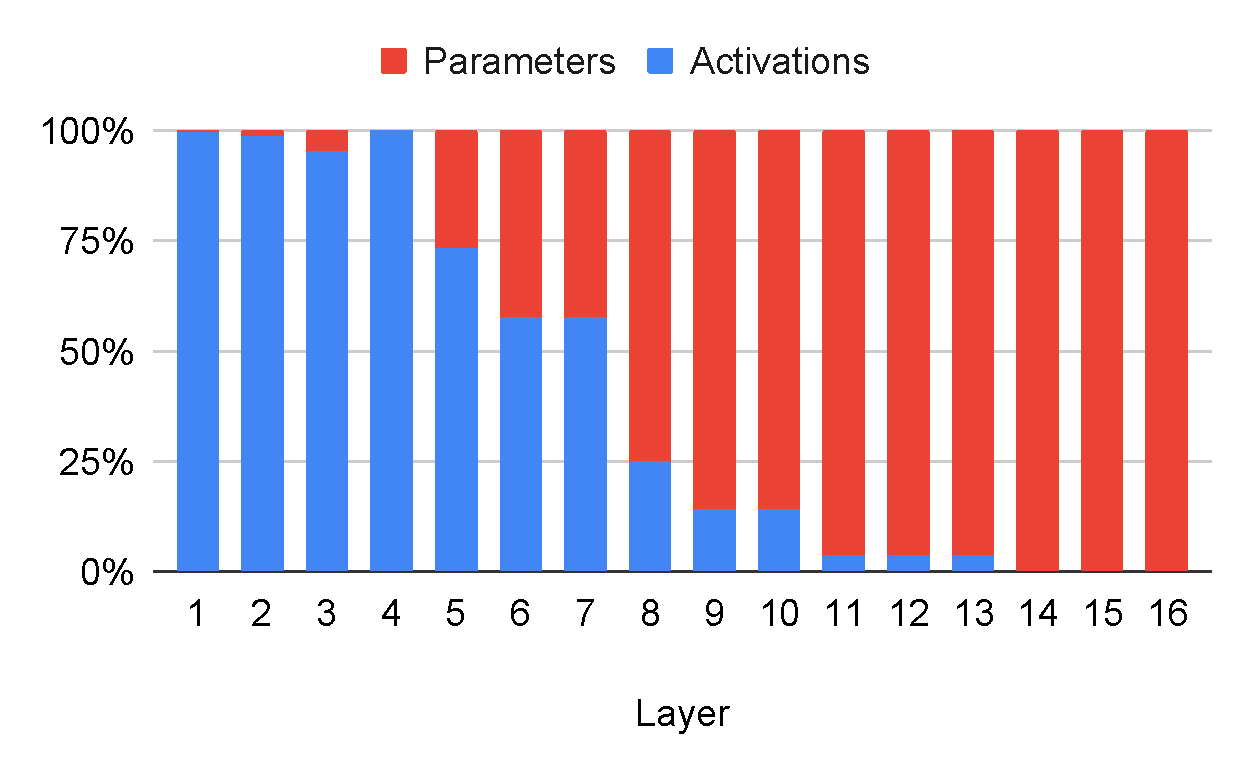
\includegraphics[width=0.49\textwidth]{VGG16ParamsNActivations}
		\label{fig:VGG16ParamsNActivations}}
	\hfil	
	\subfloat[AlexNet]{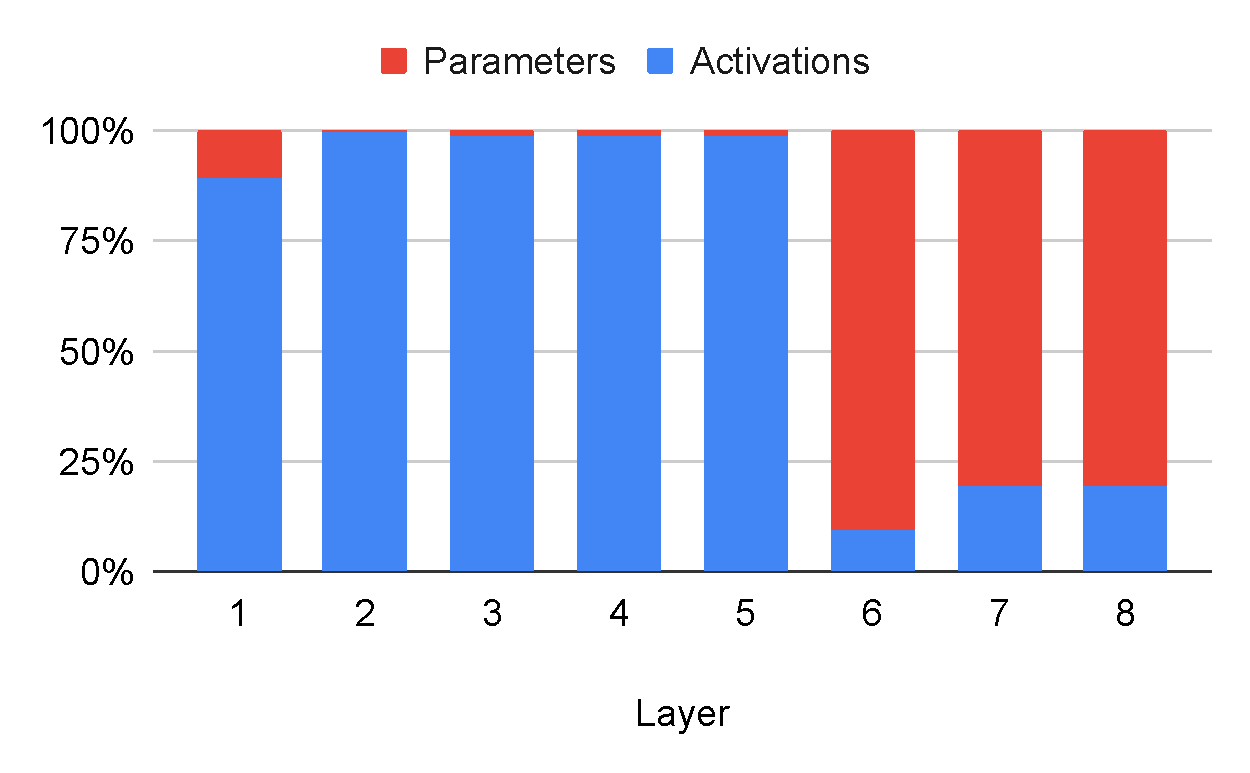
\includegraphics[width=0.49\textwidth]{AlexNetParamsNact.pdf}
		\label{fig:AlexNetParamsNact}}
	\hfil	
	\caption{Parameters and activations proportions in CL and FC layers of CNNs.}
	\label{fig:ParamsNactProp}
\end{figure}
\section{Related Work}
%Zhang et al.~\cite{zhang2015optimizing} used loop tiling to optimize the off-chip memory accesses. They expressed the off-chip memory access as a function of tile dimensions and layer shape and determined optimal tile dimensions by enumerating all the legal tile dimensions. They determined a global optimal tile dimension to reduce the hardware design complexity and used a common data reuse scheme for all the layers. Due to varying layer shapes, the optimal tile dimension and data-reuse scheme for different layers vary. To overcome this, Li et al.~\cite{Li2018SmartShuttleOO} proposed a layer-wise adaptive data partitioning and scheduling scheme. However, their approach ignored the architectural parameters and address alignment and assumed that all tiles of the same dimensions have the same off-chip memory accesses. With this assumption, the tile dimensions determined by their approaches are suboptimal.
Several studies (\cite{Li2018SmartShuttleOO, zhang2015optimizing, 7092377, MaYufei, 7302332, 7428073, 6657019}) have addressed the substantial impact of data transfer on the performance and energy efficiency of DNN accelerators. These works aimed to optimize off-chip memory accesses through techniques such as loop ordering and loop tiling.

Peeman et al.~\cite{7092377} presented an analytical method to optimize the convolution nested loops for inter-tile data reuse using loop transformations. Inter-tile reuse scheme proposed by them creates the dependencies between the tiles and reduces the inter-tile parallelism. Ma et al.~\cite{MaYufei}, opted to ignore tile overlap, utilizing a fixed loop ordering and loop tiling scheme. They stored the full depth of $ifm$ tiles to minimize partial sum access from off-chip memory, but this approach may not scale for layers with numerous feature maps.
 
Shi et al.~\cite{7302332} proposed intra-output feature map parallelism to leverage data locality, aiming to reduce off-chip DRAM accesses by reusing data from on-chip buffers. However, their design has limitations, including the use of separate buffers for input and output feature maps, reducing flexibility. Additionally, their analysis focused solely on height and width tile dimensions, employing a fixed loop ordering and tiling scheme that may not be optimal for various layer shapes in CNNs. 

Zhang et al.~\cite{zhang2015optimizing} expressed off-chip memory access as a function of tile dimensions and layer shape, determining optimal tile dimensions by enumerating legal options. They sought a global optimal tile dimension to simplify hardware design, utilizing a common data reuse scheme for all layers. However, due to varying layer shapes, the optimal tile dimensions and data-reuse schemes differ across layers.

Motamedi et al.~\cite{7428073} considered the impact of adaptive tiling and demonstrated its superior performance compared to static solutions. However, their adaptive tiling was limited to height and width dimensions of feature maps.

The closest approach to ours is the layer-wise adaptive data partitioning and scheduling scheme by Li et al.~\cite{Li2018SmartShuttleOO}. Nevertheless, their method overlooked architectural parameters and address alignment, assuming identical off-chip memory accesses for tiles of the same dimensions. This assumption may lead to suboptimal tile dimensions in their approach.

Our approach considers an adaptive strategy for loop tiling and loop orderding for all the layers, analyzing the impact of architectural parameters on off-chip memory access. We use this information to determine optimal tile dimensions and data reuse scheme, aiming to reduce off-chip memory accesses for different layers of CNNs.

\section{Off-Chip Memory Accesses of CNN Layers}\label{MemAccess_CNN}
%\subsection{Off-chip memory access of CL}\label{sec:AccessCLData}
\begin{comment}
A CNN accelerator accesses 3D data of \textit{ifm, ofm}, and \textit{wts} of each layer partitioned into tiles. It accesses tiles of the layer from off-chip memory one or multiple times. Trip counts of the tiles depend on the layer shape, tile dimensions, and the data reuse scheme. If the batch size is $D$, layer shape is $\langle W_o,H_o,N_i,M_o\rangle$ and tiling parameters are $\langle T_{c_o},T_{r_o},T_{n_i},T_{m_o}\rangle$, trip counts of tiles in IRO, ORO, and WRO schemes can be expressed as the rows of the matrix $\mathbf{R}$ in ~\eqref{eq:TripCount}, where columns represent \textit{ifm, ofm}, and \textit{wts} trip counts.
\begin{align}\label{eq:TripCount}
	\mathbf{R}=
	\begin{bmatrix}
		\mathbf{r}_{iro} \\  \mathbf{r}_{oro} \\ \mathbf{r}_{wro} \\
	\end{bmatrix}=
	\begin{bmatrix}
		D&(2\ceil[\big]{\frac{N_i}{T_{n_i}}}-1)D&\ceil[\big]{\frac{H_o}{T_{r_o}}}\ceil[\big]{\frac{W_o}{T_{c_o}}}D\\[6pt]
		\ceil[\big]{\frac{M_o}{T_{m_o}}}D&D&\ceil[\big]{\frac{H_o}{T_{r_o}}}\ceil[\big]{\frac{W_o}{T_{c_o}}} D\\[6pt]
		\ceil[\big]{\frac{M_o}{T_{m_o}}}D&(2\ceil[\big]{\frac{N_i}{T_{n_i}}}-1)D&1\\
	\end{bmatrix}
\end{align}
\end{comment}
CNN accelerators access 3D data of \textit{ifm, ofm}, and \textit{wts} of each layer partitioned into tiles. It accesses tiles of the layer from off-chip memory one or multiple times. Trip counts of the tiles depend on the layer shape, tile dimensions, and the data reuse scheme. If the batch size is $D$, layer shape is $\langle W_o,H_o,N_i,M_o\rangle$, and tiling parameters are $\langle T_{c_o},T_{r_o},T_{n_i},T_{m_o}\rangle$, trip counts of tiles in IRO, ORO, and WRO schemes can be determined using layer shape and tiling parameters. 
\subsection{Trip Counts of Tiles}\label{sec:TripCount}
\figref{fig:convPartitionedLayer} shows a toy convolution layer data partitioned into tiles. The $ifm$ is partitioned into two tiles in spatial dimension and two in depth. There are two filters $wts_C$ and $wts_D$ in the layer, and each is partitioned into two tiles in depth. The convolution output is computed and stored as 4 $ofm$ tiles.
\begin{figure}[!htb]
	\centering
	\captionsetup{font=sf}	
	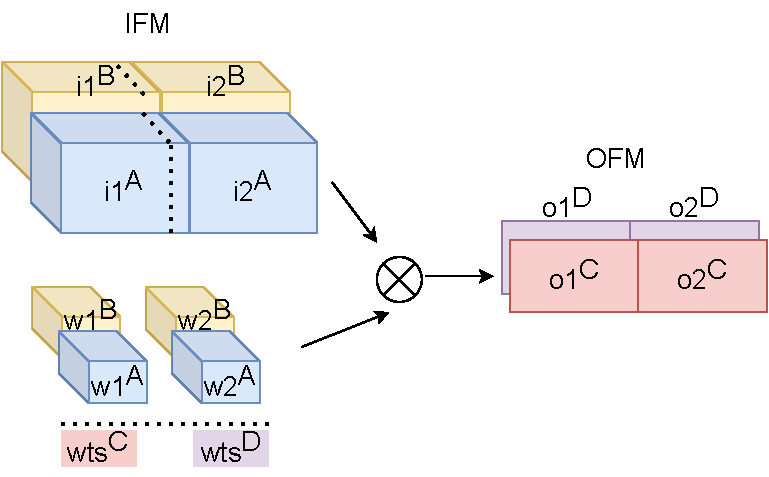
\includegraphics[width=0.7\textwidth]{Conv2by2.pdf}
	\caption{A Convolution layer data partitioned into tiles }
	\label{fig:convPartitionedLayer}
\end{figure}
\figref{fig:differentScheduling} shows three different valid schedules for the tiles of the convolution layer shown in \figref{fig:convPartitionedLayer}. 
\begin{figure}[!htb]
	\centering
	\captionsetup{font=sf}
	\subfloat[IRO Scheduling]{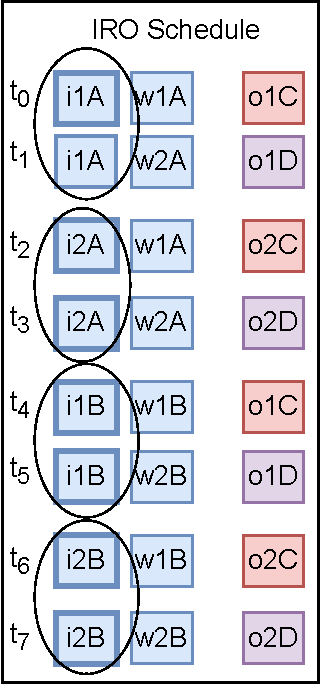
\includegraphics[width=0.25\textwidth]{IROScheduling.pdf}
	\label{fig:IROScheduling}}
    \hfil		
	\subfloat[ORO Scheduling]{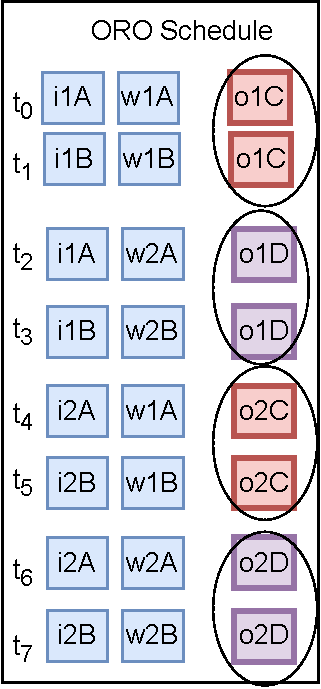
\includegraphics[width=0.25\textwidth]{OROScheduling.pdf}
		\label{fig:OROScheduling}}
	\hfil	
	\subfloat[WRO Scheduling]{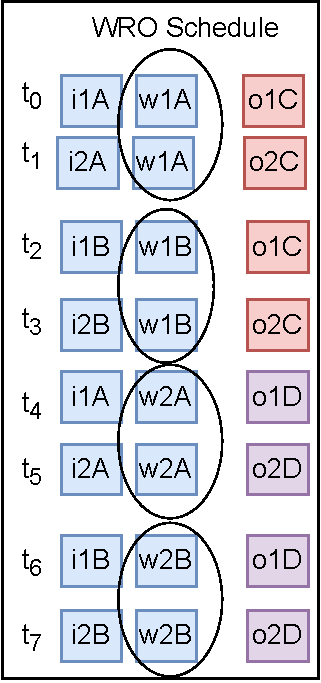
\includegraphics[width=0.25\textwidth]{WROScheduling.pdf}
		\label{fig:WROScheduling}}
	\hfil	
	\caption{Different Scheduling of tiles.}
	\label{fig:differentScheduling}
\end{figure}

There are several ways in which a  combination of $ifm$, $ofm$, and $wts$ tiles can be accessed from the off-chip memory to perform the computations by the accelerator, resulting in a valid schedule. These schedules differ in how tile combinations are fetched from the off-chip memory and the volume of off-chip memory accesses. \figref{fig:differentScheduling} shows three different schedules, which minimizes the off-chip memory accesses of one data type.

\figref{fig:IROScheduling} shows the Input Reuse Oriented (IRO) scheme schedule, which maximizes the input data reuse. In the IRO scheduling scheme, all the operations involving a given $ifm$ tile are scheduled consecutively to access each $ifm$ tile only once from the off-chip memory. There are $\ceil[\big]{\frac{H_o}{T_{r_o}}}\ceil[\big]{\frac{W_o}{T_{c_o}}}$ number of $ifm$ tiles in spatial dimension and $\ceil[\big]{\frac{N_i}{T_{n_i}}}$ number of $ifm$ tiles in depth dimension. Each $wts$ tile is accessed repeatedly from the off-chip memory to convolve with different spatial $ifm$ tiles, and each $ofm$ tile is accessed repeatedly to compute the final outputs using the $ifm$ tiles in the depth dimension. Unlike the $wts$ tile, which are only read from the off-chip memory, each $ofm$ tile needs to be written to and read from the off-chip memory, except the first time when it is only written. The trip count of $ifm$, $ofm$ and $wts$ tiles in IRO scheme can be computed as following,
\begin{align}\label{eq:IROTripCount}
	\begin{split}
	r_{ifm} &= D \\
	r_{ofm}&= (2\ceil[\big]{\frac{N_i}{T_{n_i}}}-1)D \\
	r_{wts} &= \ceil[\big]{\frac{H_o}{T_{r_o}}}\ceil[\big]{\frac{W_o}{T_{c_o}}}D
	\end{split}
\end{align}
\figurename~\ref{fig:OROScheduling} shows the Output Reuse Oriented (ORO) scheme, which maximizes the reuse of partial sums. In the ORO scheduling scheme, all the partial sums required for an $ofm$ tile are performed consecutively, and the final sum is written once to the off-chip memory. Computing a single $ofm$ tile requires convolving all the $ifm$ and $wts$ tiles in the input depth dimension. This results in repeatedly accessing the $ifm$ and $wts$ tiles from the off-chip memory. In this scheme, each $ifm$ tile is accessed $\ceil[\big]{\frac{M_o}{T_{m_o}}}$ times to convolve with all the filters and each $wts$ tile is accessed $\ceil[\big]{\frac{H_o}{T_{r_o}}}\ceil[\big]{\frac{W_o}{T_{c_o}}}$ times to perform the operations with all the $ifm$ tiles in spatial dimensions. The trip count of $ifm$, $ofm$, and $wts$ tiles for the ORO scheduling scheme can be computed as following,
\begin{align}\label{eq:OROTripCount}
	\begin{split}
		r_{ifm} &= \ceil[\big]{\frac{M_o}{T_{m_o}}}D \\
		r_{ofm}&= D \\
		r_{wts} &= \ceil[\big]{\frac{H_o}{T_{r_o}}}\ceil[\big]{\frac{W_o}{T_{c_o}}} D
	\end{split}
\end{align}
\figref{fig:WROScheduling} shows the Weight Reuse Oriented (WRO) scheme that maximizes the weights reuse. Each $wts$ tile is accessed once from the off-chip memory, and all the operations involving the $wts$ tile are performed consecutively. This requires repeatedly accessing the $ifm$ and $ofm$ tiles from the off-chip memory. Each $ifm$ tile  is accessed $\ceil[\big]{\frac{M_o}{T_{m_o}}}$ times, once for each $wts$ tile. There are $\ceil[\big]{\frac{N_i}{T_{n_i}}}$ tiles in the input depth. The partial sums resulting from each $ifm$ tile in the input depth need to be read from and written to off-chip memory, except for the first tile, which is only written to the off-chip memory. Total trip counts of the output partial sums tiles are $(2\ceil[\big]{\frac{N_i}{T_{n_i}}}-1)$. In this case, the trip count of $ifm$, $ofm$ and $wts$ tiles can be computed as following,
\begin{align}\label{eq:WROTripCount}
	\begin{split}
		r_{ifm} &= \ceil[\big]{\frac{M_o}{T_{m_o}}}D\\
		r_{ofm}&= (2\ceil[\big]{\frac{N_i}{T_{n_i}}}-1)D \\
		r_{wts} &= 1
	\end{split}
\end{align}
Trip counts of $ifm$, $ofm$, and $wts$ tiles in IRO, ORO, and WRO schemes can be expressed as the rows of the matrix $\mathbf{R}$ using~\eqref{eq:IROTripCount},~\eqref{eq:OROTripCount}, and~\eqref{eq:WROTripCount}, where columns represent \textit{ifm, ofm}, and \textit{wts} trip counts as shown in~\eqref{eq:TripCount} below.
\begin{align}\label{eq:TripCount}
	\mathbf{R}=
	\begin{bmatrix}
		\mathbf{r}_{iro} \\  \mathbf{r}_{oro} \\ \mathbf{r}_{wro} \\
	\end{bmatrix}=
	\begin{bmatrix}
		D&(2\ceil[\big]{\frac{N_i}{T_{n_i}}}-1)D&\ceil[\big]{\frac{H_o}{T_{r_o}}}\ceil[\big]{\frac{W_o}{T_{c_o}}}D\\[6pt]
		\ceil[\big]{\frac{M_o}{T_{m_o}}}D&D&\ceil[\big]{\frac{H_o}{T_{r_o}}}\ceil[\big]{\frac{W_o}{T_{c_o}}} D\\[6pt]
		\ceil[\big]{\frac{M_o}{T_{m_o}}}D&(2\ceil[\big]{\frac{N_i}{T_{n_i}}}-1)D&1\\
	\end{bmatrix}
\end{align}
\subsection{Off-chip memory access of CL}\label{sec:AccessCLData}
To compute the off-chip memory accesses for a CL layer, first, we compute the off-chip memory accesses for one trip of $ifm$, $ofm$ and $wts$ using~\algref{Algorithm1} of~\chapref{chap:analyticalFw} as below
\begin{align}\label{eq:MemAccessCL}
	\begin{split}
		\numBytesOffChip_{ifm}=&\emph{BWA}(\addressSym_{ifm},\langle T_{c_i}, T_{r_i},T_{n_i}\rangle,\langle W_i,H_i,N_i\rangle,\numOverlap)\\
		\numBytesOffChip_{ofm}=&\emph{BWA}(\addressSym_{ofm},\langle T_{c_o},T_{r_o},T_{m_o}\rangle,\langle W_o,H_o,M_o\rangle,0)\\
		\numBytesOffChip_{wts}=&M_o\cdot \emph{BWA}(\addressSym_{wts},\langle K,K,T_{n_i}\rangle,\langle K,K,N_i\rangle,0)
	\end{split}
\end{align} 
where $\numOverlap=(K-S)$ is the number of overlapping elements between adjacent $ifm$ tiles. $\numBytesOffChip_{ifm}$, $\numBytesOffChip_{ofm}$, and $\numBytesOffChip_{wts}$ are the number of bytes accessed from off-chip memory for one trip of \textit{ifm, ofm} and \textit{wts} respectively. $\langle W_{i},H_{i},N_{i}\rangle$ are the \textit{ifm} data shape and $\langle T_{c_i},T_{r_i},T_{n_i}\rangle$ are the \textit{ifm} tile dimensions. \textit{ofm} layer shape $\langle W_{o},H_{o},M_{o}\rangle$ is computed using~\eqref{eq:ifmOfmStrideS_P} and $ofm$ tile dimensions can be computed using~\eqref{eq:ifmOfmStrideS_P} as below,
\begin{align}\label{eq:ofmAndifmTileDims}
	\begin{split}
		T_{c_o}&=\frac{T_{c_{i}}-K}{S}+1 \\
		T_{r_o}&=\frac{T_{r_{i}}-K}{S}+1,
	\end{split}
\end{align}  
The total number of bytes accessed for j$^{th}$ reuse scheme ($\numBytesOffChip_j$) can be expressed as following sum
\begin{equation} \label{eq:TotalOffChipAccess}
	\numBytesOffChip_j=\mathbf{r_j}\cdot \begin{bmatrix}
		\numBytesOffChip_{ifm} &
		\numBytesOffChip_{ofm} &
		\numBytesOffChip_{wts}
	\end{bmatrix}^{T}
\end{equation}
where \textbf{r}$_j$ is the row vector of the matrix $\mathbf{R}$ (\eqref{eq:TripCount}) for the j$^{th}$ scheme. 
\subsection{Optimization problem}
Now, we present determining the optimal tile dimensions as a constraint optimization problem. Tiles of \textit{ifm, ofm} and \textit{wts} reside in on-chip memory. The volume of the tiles is given by equation~\eqref{eq:tilesVol} below,
\begin{align}\label{eq:tilesVol}
	\begin{bmatrix}
		V_i \\ V_o \\ V_w
	\end{bmatrix}=
	\begin{bmatrix}
		T_{c_i}\cdot T_{r_i}\cdot T_{n_i}\\
		T_{c_o}\cdot T_{r_o}\cdot T_{m_o}\\
		K^2\cdot T_{n_i}\cdot T_{m_o}\\
	\end{bmatrix}
\end{align}
where $V_i, V_o, \text{and }V_w$ are the sizes of \textit{ifm, ofm}, and \textit{wts} tiles, respectively. If the on-chip memory buffer size is $\BuffSize$ and each data element is represented by $\dataWidth$ bytes, then constraints on tile dimensions are
\begin{align}\label{eq:onChipConstraint}
	\begin{split}
		&(V_i + V_w + V_o)\cdot \dataWidth\leq \BuffSize \\
		&0<T_{c_o}\leq W_o,~\ 0<T_{r_o}\leq H_o\\
		&0<T_{n_i}\leq N_i,~\ 0<T_{m_o}\leq M_o
	\end{split}
\end{align}
Determining the tile dimensions which minimize the off-chip memory accesses, expressed by \eqref{eq:TotalOffChipAccess}, is a constraint optimization problem. The  number of bytes accessed from off-chip memory using j$^{th}$ reuse scheme $\numBytesOffChip_j$ (~\eqref{eq:TotalOffChipAccess}) and the constraints (~\eqref{eq:onChipConstraint}) are non-linear functions of four variables $\langle T_{c_o},T_{r_o},T_{n_i},T_{m_o}\rangle$, and thus solving it is non-trivial.
\subsection{Off-chip memory access of FCL}\label{sec:AccessFCLData}
The computations of FCLs are a special case of CLs with additional constraints on layer shapes and parameters. The \textit{ifm} volume is same as a filter volume i.e., $H_i{=}W_i{=}K$, padding $P{=}0$, and stride $S{=}1$. In CNNs, typical values of K are 1, 3, 5, 7, and 11. Due to small values of $H_i$ and $W_i$, these dimensions are not partitioned ($T_{r_i}{=}T_{c_i}{=}K$). \textit{ofm} layer shape and tile dimensions computed using ~\eqref{eq:ofmAndifmTileDims} are $\langle 1,1,M_o\rangle$ and $\langle 1,1,T_{m_o}\rangle$.

For FCLs, the trips count of different data reuse schemes can be computed using~\eqref{eq:TripCount} and the number of bytes accessed from off-chip memory ($\numBytesOffChip^{FC}$) using~\eqref{eq:TotalOffChipAccess} by applying the layer shape constraints. The constraints on tile dimensions are given by~\eqref{eq:onChipConstraint}. $T_{n_i}$ and $T_{m_o}$ are the unknowns to be determined in~\eqref{eq:TotalOffChipAccess}. Determining the optimal tile dimensions for FCLs is a constraint optimization problem similar to CL.
\section{Implementation and Results}
\subsection{Implementation}
The optimal tile dimensions need to be determined once for a given NN and accelerator architecture, before the inference phase on edge devices. It can be determined by computing the number of bytes accessed from off-chip memory ($\numBytesOffChip$) at all the feasible points in the solution space. 
We have developed a tool that determines the optimal tile dimensions of each NN layer during the \emph{Preprocessing and Optimization} phase before the inference phase (~\figref{fig:workFlow} of~\chapref{chap:introduction}). The tool first prunes the large search space of tiles by applying the constraints (~\eqref{eq:onChipConstraint}). It then computes $\numBytesOffChip$ using \eqref{eq:TotalOffChipAccess} for each tile in the pruned search space and determines the optimal tile dimensions. The optimal tile dimension is determined for all the CL and FC layers of the NN. The tool also analyses the $\numBytesOffChip$ for different data reuse schemes to suggest the best scheme for each CL. It can be configured for different on-chip memory sizes, bus widths, and data bit widths. It took few minutes to determine the optimal solution for VGG16 on Intel Core i7-6700 CPU (@3.40GHz$\times$8).
\subsection{Validation}\label{Validation}
We have validated the number of bytes accessed from off-chip memory computed by BWA (~\algref{Algorithm1} of~\chapref{chap:analyticalFw}) using the hardware implementation of CNN layers on Xilinx FPGA. We have implemented CNN layers using the Xilinx SDSoC framework, SDx v2018.3, which generates hardware functions from high-level languages like C/C++. We used the SDx pragmas to use zero\_copy as a data mover. The Xilinx tools allow integrating the AXI Performance Monitor (APM) IP~\cite{APM}, which captures the real-time performance metrics like bus latency and amount of memory traffic for connected AXI interfaces. The target platform is ZedBoard, working at 100MHz frequency, and off-chip memory (DRAM) is accessed using 64 bits AXI bus. 
Our FPGA implementation takes the 3D shape and tile dimensions as input, and the generated hardware functions access the 3D data from DRAM using loop tiling. The integrated APM IP logs the number of bytes and latency of off-chip memory access transactions using which we validated the number of bytes accessed from off-chip memory computed by our approach for different 3D data shapes and tile dimensions.
\subsection{Benchmarks}
We carried out experiments on three popular CNN networks, VGG16~\cite{simonyan2014very}, AlexNet~\cite{krizhevsky2012imagenet}, and ResNet~\cite{he2016deep} having 8, 16, and 50 layers, respectively. These CNNs have varying shapes and use filters of dimensions $1{\times}1$, $3{\times}3$, $5{\times}5$, $7{\times}7$, and $11{\times}11$. To compare the results with other approaches, we have used the on-chip buffer size of 108 KB, batch size of 3 for VGG16, and 4 for ResNet and AlexNet, as used by Eyeriss~\cite{chen2016eyeriss} and SmartShuttle~\cite{Li2018SmartShuttleOO}. 
\subsection{Baselines}
We have implemented the SmartShuttle (SS)~\cite{Li2018SmartShuttleOO} approach to compare the results with our bus width aware (BWA) approach. SS statically determines the partitioning and scheduling scheme for each layer. It performs better than strategies that use a fixed tile dimension and data reuse scheme for all layers, e.g., Eyeriss~\cite{chen2016eyeriss} and  Zhang~\cite{zhang2015optimizing}. 
\subsection{Results}
\begin{figure}[!htb]
	\centering
	\subfloat[$\numBytesOffChip_{VGG16}$]
	{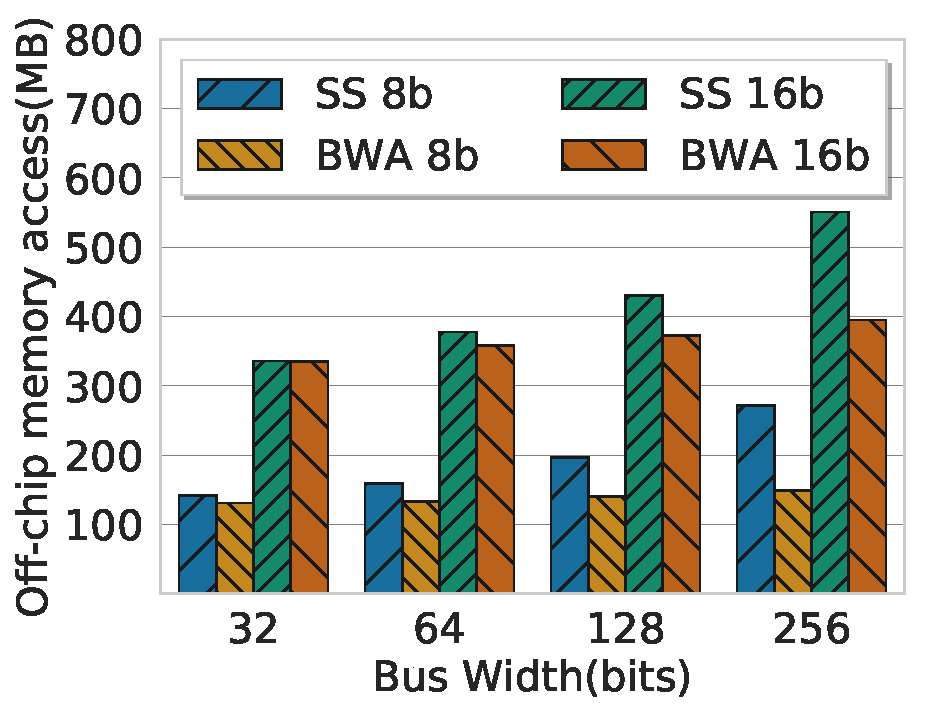
\includegraphics[width=0.32\textwidth]{VGG16_mem108_batch4_bw0_dW0_AD0.pdf}
		\label{fig:VGG16OffChipAccesses}}
	\hfil	
	\subfloat[$\numBytesOffChip_{AlexNet}$]
	{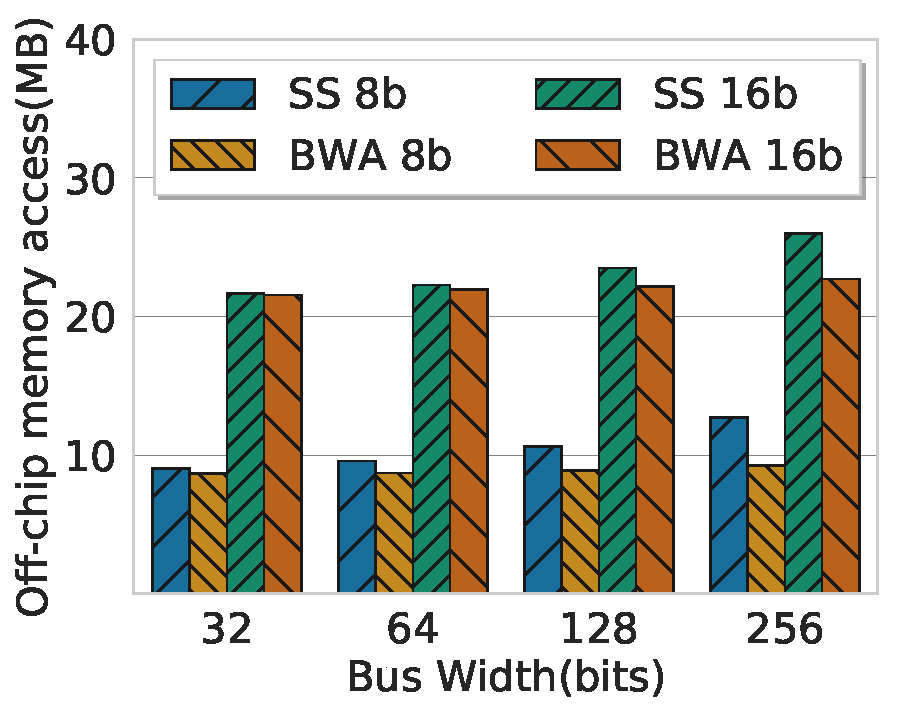
\includegraphics[width=.32\textwidth]{AlexN_mem108_batch4_bw0_dW0_AD0.pdf}
		\label{fig:AlexNetOffChipAccesses}}
	\hfil			
	\subfloat[$\numBytesOffChip_{ResNet}$]
	{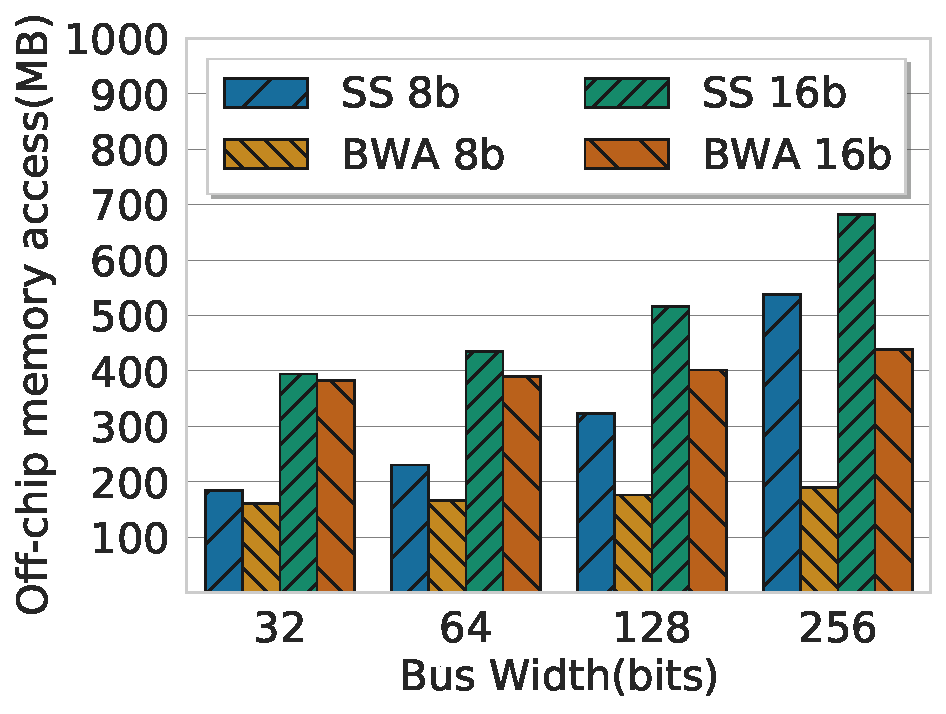
\includegraphics[width=.32\textwidth]{RESNet_mem108_batch4_bw0_dW0_AD0.pdf}
		\label{fig:ResNetOffChipAccesses}}
	\hfil	
	\caption{Off-chip memory access of convolution layers for 8 and 16 bits data width. BWA: Bus Width Aware, SS: SmartShuttle}
	\label{fig:AccessenOn64BitDataBus}
	\vspace{-1.0em}
\end{figure}
\subsubsection{Impact of Bus Width on memory access of CLs}
\figref{fig:AccessenOn64BitDataBus} shows the number of bytes accessed from off-chip memory ($\numBytesOffChip$) of CLs of the CNNs for different bus widths for 8 and 16 bits data width and 108 KB on-chip buffer size. Data is accessed in multiple of bus widths, and when the data length is not a multiple of the bus width, it leads to inefficient use of bus bandwidth. This inefficiency is more pronounced for wider data buses. For example, accessing 20 bytes on both 8-byte and 16-byte wide data buses results in 24 and 32 bytes of off-chip memory accesses, respectively. Consequently, the advantages of the BWA approach are more noticeable on wider data buses compared to narrower ones, as shown in~\figref{fig:AccessenOn64BitDataBus}. The BWA approach reduces bus width's impact on off-chip memory accesses, as it selects the tile dimensions considering the bus width and address alignments. Whereas tile dimensions selected by SS remain the same, irrespective of the bus width of the accelerator, which results in a large value of $\numBytesOffChip$.
As shown in~\figref{fig:AccessenOn64BitDataBus}, BWA reduces $\numBytesOffChip$ compared to SS for the three CNNs. For ResNet:50 it reduces $\numBytesOffChip_{ResNet}$ by 13\%, 28\%, 46\%, and 65\% for 8 bits data width and by 10\%, 22\% and 36\% for 16 bits data width on 64, 128, and 256 bits wide data bus, respectively, compared to SS. 
BWA reduces $\numBytesOffChip_{VGG16}$ by 8\%, 16\%, 29\%, and 45\% and $\numBytesOffChip_{AlexNet}$ by 4\%, 9\%, 16\% and 27\% on 32, 64, 128, and 256 bits wide buses respectively, for 8 bits data width. 
The impact of bus width is significant when accessing low-resolution data on a wide data bus. For 16 bits data width, the effectiveness of the BWA approach is noticeable for 64 or wider data buses. For 16 bits data width, BWA reduces $\numBytesOffChip_{VGG16}$ by 5\%, 13.5\% and 28\% and $\numBytesOffChip_{AlexNet}$ by 1.5\%, 5.7\% and 13\% compared to SS on 64, 128, and 256 bits wide data bus, respectively.
\subsubsection{Off-Chip Memory Access of Data Reuse  Schemes}\label{sec:ResultsDataReuseScheme}
\begin{figure}[htb]
	\centering
	\subfloat[VGG16 CLs]
	{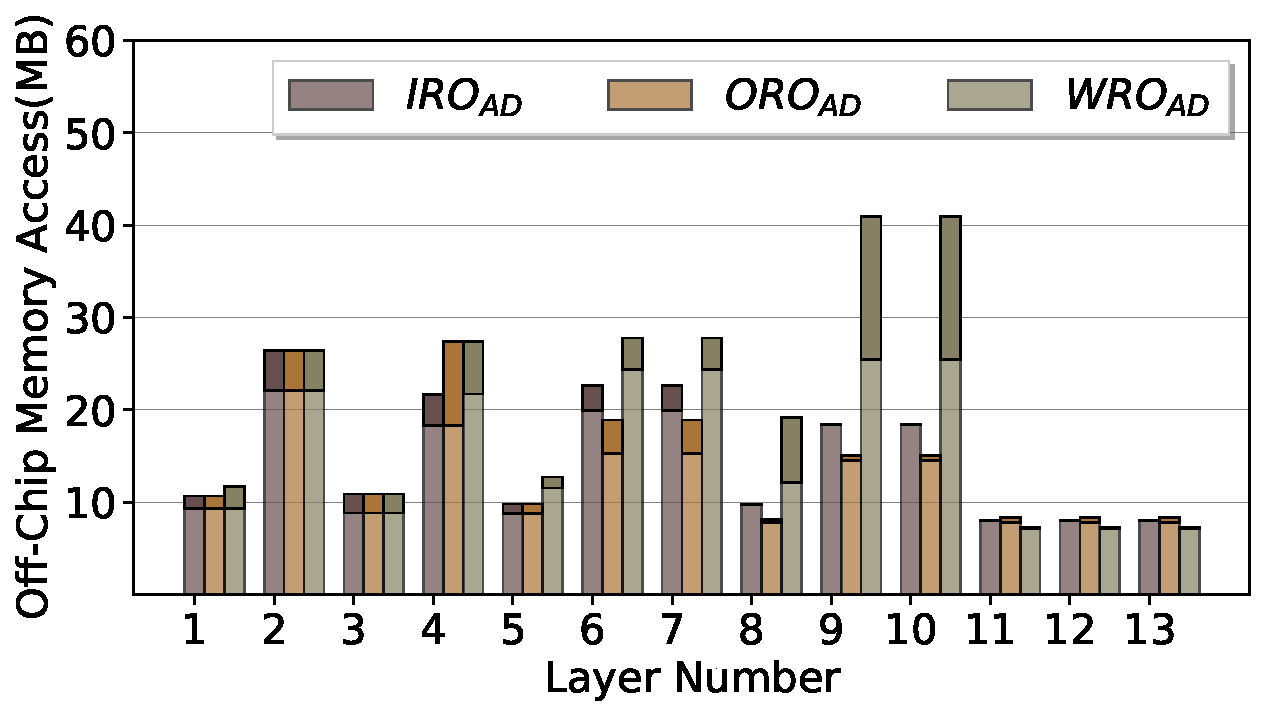
\includegraphics[width=0.48\textwidth]{VGG16_mem108_batch3_bw8_8bits_reuseSch.pdf}
		\label{fig:VGG16ReuseSchCompare}}
	\hfil
	\subfloat[AlexNet CLs]
	{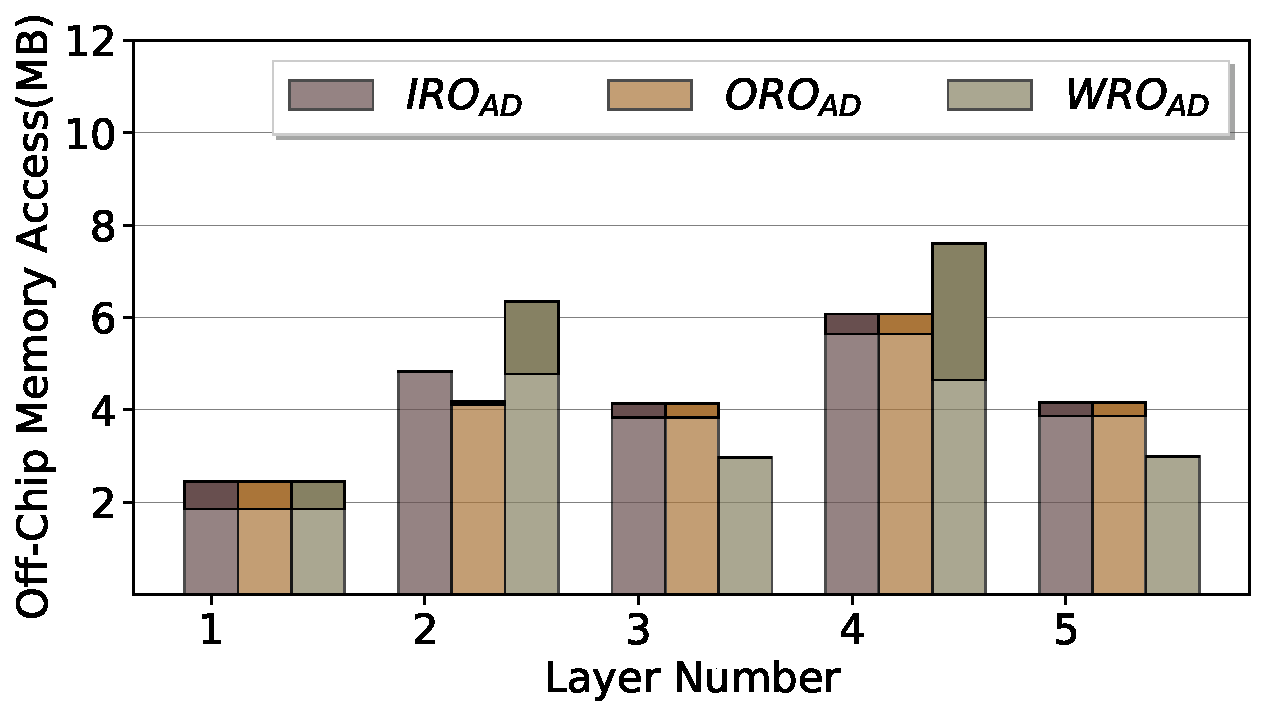
\includegraphics[width=0.48\textwidth]{AlexN_mem108_batch4_bw8_8bits_reuseSch.pdf}
		\label{fig:AlexNetReuseSchCompare}}
	\hfil	
	\caption{Layer wise off-chip memory access for IRO, ORO and WRO schemes.}
	\label{fig:DataReuseSchemeCompare}
	\vspace{-1.0em}	
\end{figure}
\figref{fig:DataReuseSchemeCompare} shows the layer-wise off-chip memory access of CLs of VGG16 and AlexNet for the three data reuse schemes using 64 bits wide bus and 8 bits data width. The results show that a single data reuse scheme is not optimal for all the layers. IRO and ORO perform better than the WRO scheme in the first few layers, while in the last few layers, WRO outperforms the other two schemes. The solid color at the top of the bars shows the reduction in off-chip memory accesses when optimal tile dimensions are selected using the BWA approach compared to when tile dimensions are selected using the tile size-based approach used by SS. For a data width of 8 bits, BWA achieves reductions of 7\%, 11\%, and 16\% in $\numBytesOffChip_{VGG16}$ and 34\%, 34\%, and 16\% in $\numBytesOffChip_{AlexNet}$ when compared to SS. These improvements are observed for IRO, ORO, and WRO reuse schemes, respectively, on a 64-bit-wide data bus.
\subsubsection{On-chip Buffer Size}
\begin{figure}[htb]
	\centering
	\subfloat[$\numBytesOffChip_{VGG16}$]
	{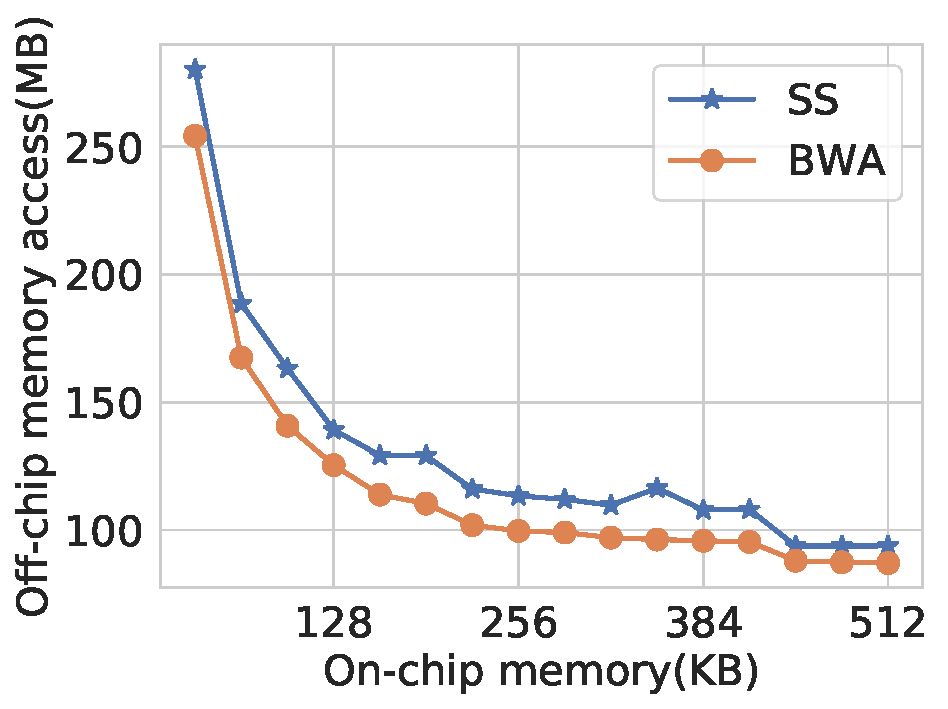
\includegraphics[width=0.42\textwidth]{VGG16_mem0_batch3_bw8_dW8_AD0.pdf}
		\label{fig:VGG16OnChipMemoryEffect}}
	\hfil
	\subfloat[$\numBytesOffChip_{AlexNet}$]
	{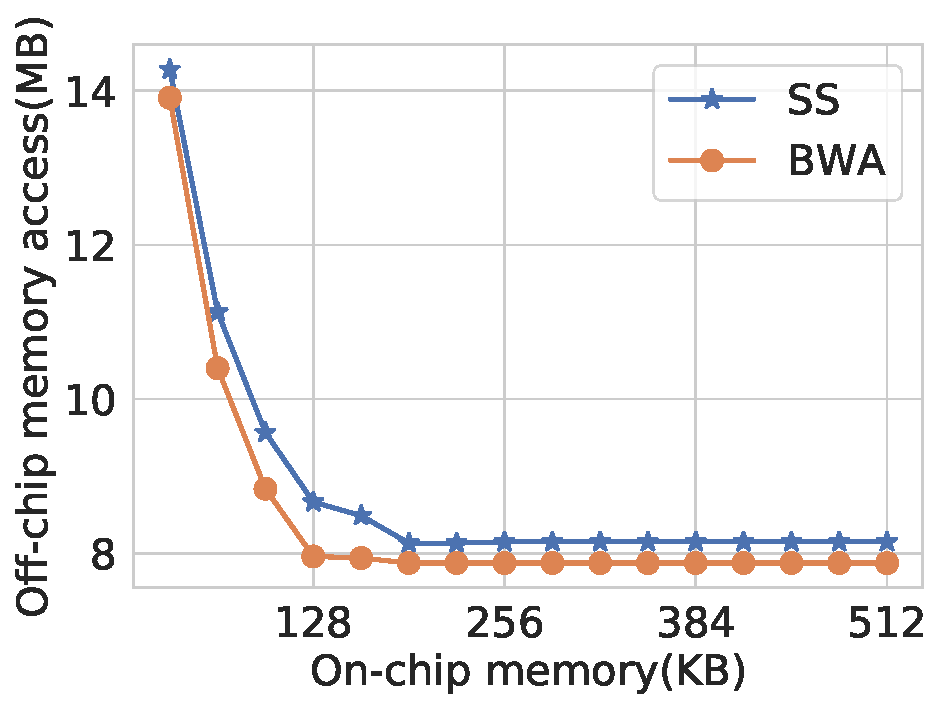
\includegraphics[width=0.42\textwidth]{AlexN_mem0_batch4_bw8_dW8_AD0.pdf}
		\label{fig:AlexNOnChipMemoryEffect}}
	\hfil
	\caption{Off-chip memory access for varying on-chip buffer sizes. BWA: Bus Width Aware, SS:SmartShuttle}
	\label{fig:EffectOfVaryingOnChipBuffer}
	\vspace{-1.0em}
\end{figure}
\figref{fig:VGG16OnChipMemoryEffect} and \figref{fig:AlexNOnChipMemoryEffect} compares the number of bytes accessed from off-chip memory ($\numBytesOffChip$) for different on-chip buffer sizes ($\BuffSize$) for VGG16 and AlexNet, respectively. A large on-chip buffer can accommodate larger tiles, which reduces the tiles' trip counts (~\eqref{eq:TripCount}) and, therefore, the total off-chip memory accesses of the CNN (~\eqref{eq:TotalOffChipAccess}). This behavior is observed for both the CNNs in~\figref{fig:VGG16OnChipMemoryEffect} and~\figref{fig:AlexNOnChipMemoryEffect}. Both approaches select the dimensions of the tiles with the constraints of on-chip buffer size. However, the proposed BWA approach performs better as it considers address alignments and bus width to reduce unwanted data transfers and optimize off-chip memory accesses. In contrast, the SS approach ignores the architectural parameters.
\subsubsection{Impact of Bus Width on $\numBytesOffChip$ of FCLs}
\begin{figure}[htb]
	\centering
	\subfloat[VGG16]
	{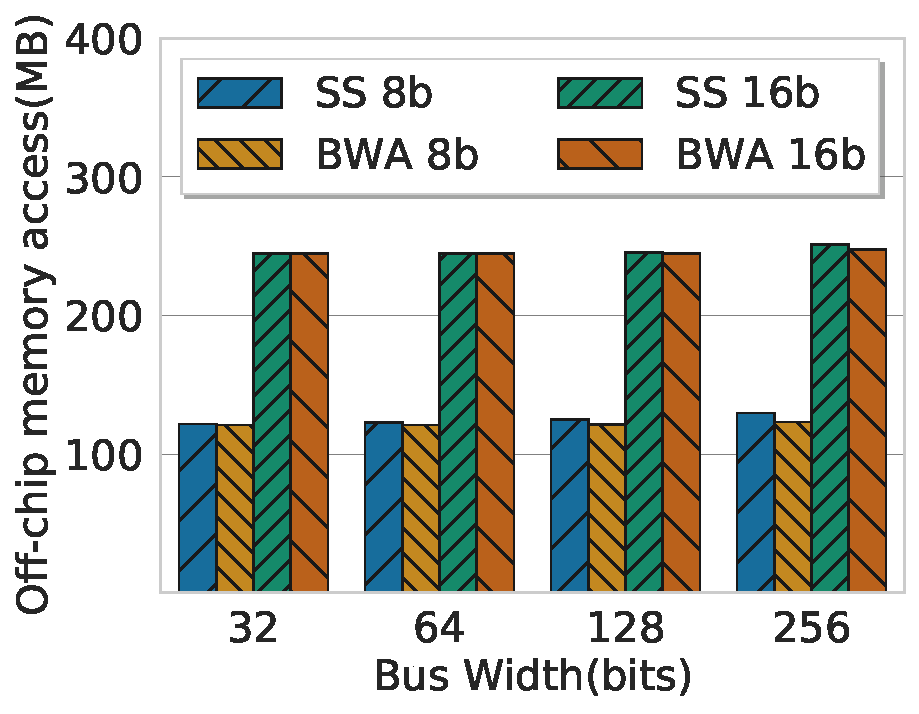
\includegraphics[width=0.4\textwidth]{VGG16_mem108_batch3_bw0_dW0_AD0_FC.pdf}
		\label{fig:VGG16FCLayer}}
	\hfil
	\subfloat[AlexNet]
	{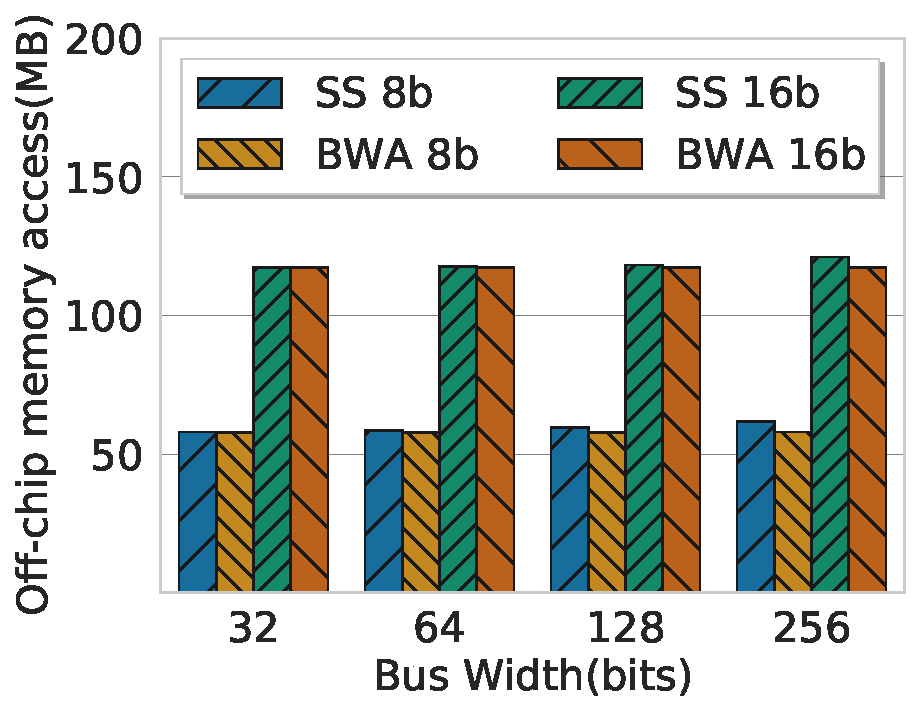
\includegraphics[width=0.4\textwidth]{AlexN_mem108_batch4_bw0_dW0_AD0_FC.pdf}
		\label{fig:AlexNetFCLayer}}
	\hfil	
	\caption{Off-chip memory access of Fully connected layers. BWA: Bus Width Aware, SS:SmartShuttle}
	\label{fig:EffectOnFC}
	\vspace{-1.0em}
\end{figure}
In fully connected (FC) layers, spatial dimensions (height and width) are notably smaller compared to convolutional (CL) layers. For instance, the spatial dimensions of the last two FC layers in VGG16 are $1{\times}1$, whereas the spatial dimensions of the first two CL layers are $224{\times}224$. When tiling the spatial dimensions of CLs, a large number of unaligned accesses occur, unlike in FC layers where such unaligned accesses are absent. The absence of tiling in FC layers for spatial dimensions reduces the occurrence of unaligned accesses. Consequently, the advantages of the bandwidth (BW) approach on $\numBytesOffChip$ are not as significant in FC layers compared to CL layers. \figref{fig:VGG16FCLayer} and~\figref{fig:AlexNetFCLayer} shows the off-chip memory accesses of FCLs of VGG16 and AlexNet, respectively, for 8 bits data width. BWA reduces $\numBytesOffChip_{VGG16}^{FC}$ by 1\%, 2\%, 3\%, and 4\% and $\numBytesOffChip_{AlexNet}^{FC}$ by 0.2\%, 1\%, 3\% and 6\% on 32, 64, 128, and 256 bits wide buses, respectively.
\subsubsection{Latency And Energy Analysis}
\begin{figure}[htb]
	\centering
	\subfloat[VGG16]
	{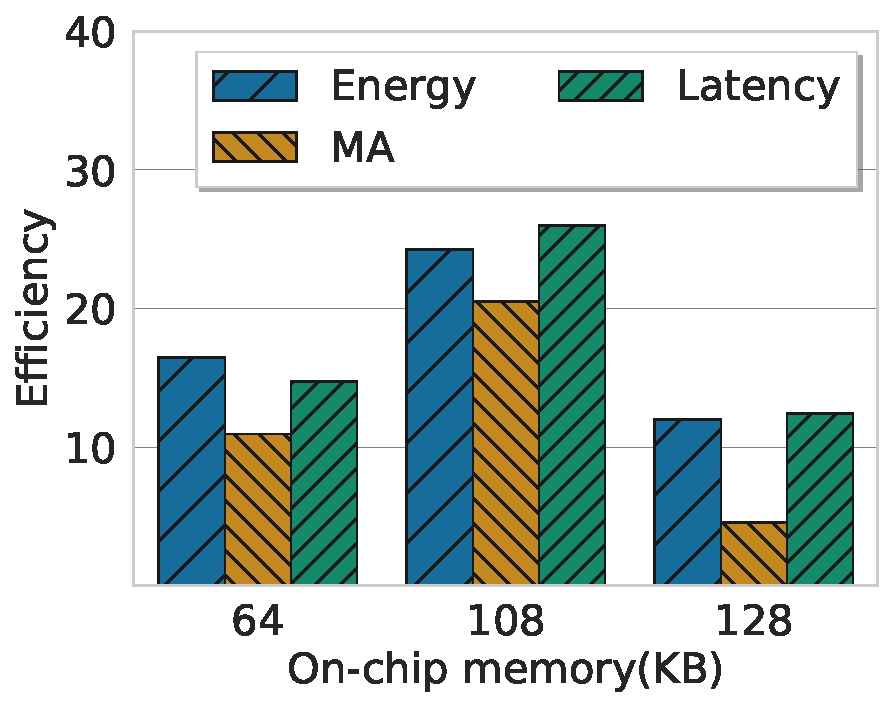
\includegraphics[width=0.4\textwidth]{energy_VGG16_DW8_BW64.pdf}
		\label{fig:VGG16EnergyEfficiency}}
	\hfil
	\subfloat[AlexNet]
	{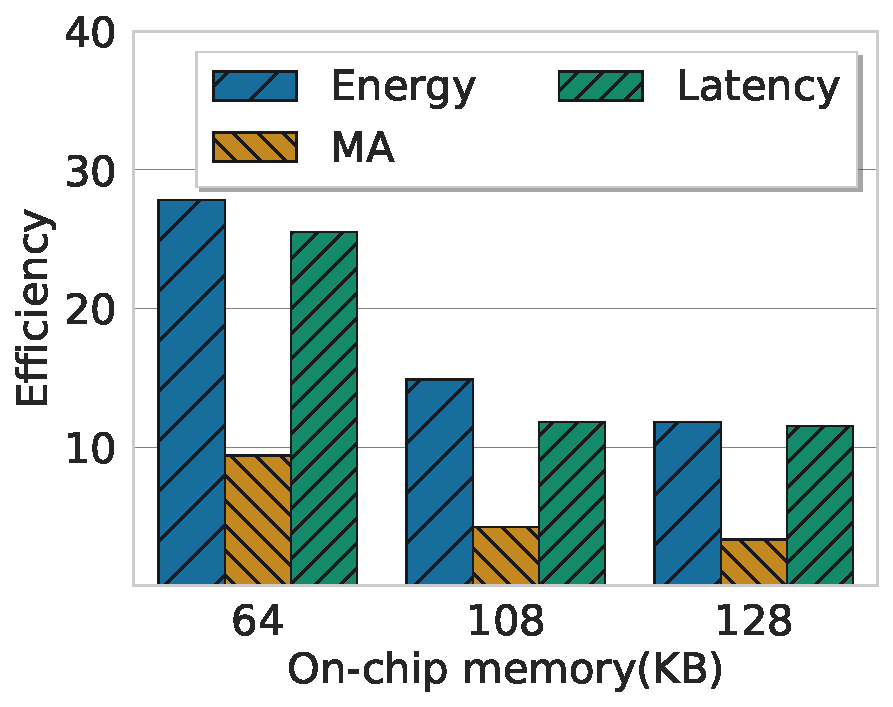
\includegraphics[width=0.4\textwidth]{energy_Alex_DW8_BW64.pdf}
		\label{fig:AlexEnergyEfficiency}}
	\hfil
	\caption{Energy and latency efficiency. BWA: Bus Width Aware, SS:SmartShuttle}
	\label{fig:EffectOnLatency}
	\vspace{-1.0em}
\end{figure}
Using our FPGA implementation, we measured the memory access latencies and execution time for CLs for the optimal tile dimensions determined using the approach described in \secref{MemAccess_CNN}. To estimate the energy efficiency achieved by the BWA compared to the SS approach, we computed the energy consumption using the following equation~\cite{tu2017deep}
\begin{align}\label{eq:energyEfficiency}
	E~{=}~P\cdot Time~{+}~\numBytesOffChip\cdot E_{DDR}
\end{align}
where $P$ is the FPGA design power reported by the Vivado synthesis tool, $Time$ is the execution time, $\numBytesOffChip$ is the number of bytes accessed from off-chip memory logged using Xilinx APM IP, and $E_{DDR}$ is the off-chip memory access energy per bit. We have used $E_{DDR}$=70 pJ/bit, a typical value for the DDR3 memory access energy~\cite{6237004}.

\figref{fig:VGG16EnergyEfficiency} and \figref{fig:AlexEnergyEfficiency} show the energy, off-chip memory accesses, and latency efficiency achieved using the BWA compared to the SS approach for VGG16 and AlexNet, respectively, for 8 bits data width and 64 bits bus width. We observed that the changes in energy and latency are proportional to the changes in memory access. This observation confirms that off-chip memory access dominates the energy consumption of the CNN accelerators. 
\section{Summary}
Off-chip memory accesses dominate the energy consumption of CNN accelerators. Loop tiling is a common technique to partition the layer data into smaller tiles that fit into on-chip memory. The tile dimensions significantly impact the off-chip memory accesses of these accelerators. In this work, we propose a bus width and address alignment aware approach to compute the off-chip memory accesses of 3D data. Our tool statically analyses the memory accesses to find the optimal tile dimensions for CNN accelerators. Experimental results show that our approach reduces off-chip memory accesses of the CLs of VGG16 by 16\%, 29\%, and of AlexNet by 9\%, 16\% on 64 and 128 bits data bus, respectively, for 8 bits data width, compared to the state-of-the-art approach.